\documentclass{article}
\usepackage{hyperref}
\usepackage{listings}
\usepackage{color}
\usepackage{xcolor}
\usepackage{geometry}
\usepackage{graphicx}
\usepackage{amsmath}
\usepackage{caption}
\usepackage{subcaption}
\geometry{margin=1in}
\pdfminorversion=6

\newcommand\TODO[1]{\textcolor{red}{TODO: #1}}

\newcommand\header[2]{
    \begin{center}
        {\large
        UCSD CSE 168 Assignment #1: \\
        \vspace{0.3cm}
        \Large
        #2}
    \end{center}
}

\definecolor{dkgreen}{rgb}{0,0.6,0}
\definecolor{gray}{rgb}{0.5,0.5,0.5}
\definecolor{mauve}{rgb}{0.58,0,0.82}
\lstset{frame=tb,
        aboveskip=3mm,
        belowskip=3mm,
        showstringspaces=false,
        columns=flexible,
        basicstyle={\small\ttfamily},
        numbers=none,
        numberstyle=\tiny\color{gray},
        keywordstyle=\color{blue},
        commentstyle=\color{dkgreen},
        stringstyle=\color{mauve},
        breaklines=true,
        breakatwhitespace=true,
        tabsize=2
}

\hypersetup{colorlinks=true}

\usepackage{xcolor}

\begin{document}

\header{3}{Textures, shading normals, area lights, and BRDFs}

In the previous homework, we mostly focused on increasing the \emph{geometric complexity} of our renderer and scenes. In this homework, we're going to implement a bunch of small features for our renderer to increase the \emph{material} and \emph{lighting complexity} of our scenes. We will still stay in the \href{https://raytracing.github.io/books/RayTracingTheNextWeek.html}{Ray Tracing - The Next Week (RTNW)} book for this homework.

\section{Textures}
So far, we assume constant color per object. This is kind of boring and real world objects are {\color{red}c}{\color{orange}o}{\color{green}l}{\color{blue}o}{\color{cyan}r}f{\color{magenta}u}{\color{violet}l}. The way computer graphics deal with colors on objects is through \href{https://en.wikipedia.org/wiki/Texture_mapping}{textures} (invented by Edwin Catmull in the 70s!): basically we wrap an image around a surface and define color on that image. There are two common ways to specify a texture: you can specify it \emph{procedurally} through a program, or you can use a raster image to represent the texture. We will implement the raster image texture, and the procedural texture will be bonus.

Go read \href{https://raytracing.github.io/books/RayTracingTheNextWeek.html#solidtextures}{Chapter 4} and \href{https://raytracing.github.io/books/RayTracingTheNextWeek.html#imagetexturemapping}{Chapter 6} of RTNW.

For the UV coordinates, we will use the same as the RTNW book for spheres. For triangles, there are two possiblities. First, the triangle mesh can come with its own UV coordinates per triangle vertex. You can access it through \lstinline{ParsedTriangleMesh::uvs} -- if the mesh contains UV coordinates, \lstinline{uvs} would be an array with the same size as \lstinline{positions}. To get the UV coordinates at each point, we interpolate from the three UV values from the vertices using the barycentric coordinates $(s, t)$: $u = (1 - s - t)u_0 + s * u_1 + t * u_2$.
Second, if the triangle mesh does not come with UV coordinates (\lstinline{uvs.size() == 0}), we will just use the barycentric coordinates $(s, t)$ as our UV.

When looking up the texture given a UV coordinate, we will do something different from the RTNW book. Firstly, the RTNW book \emph{clamps} the UV coordinates when they are smaller than 0 or larger than 1. This is not ideal when we want to tile the textures and repeat them across the surface. Instead, we will wrap the UV coordinates around by taking a \lstinline{modulo} by one. For example, if $u = 1.5$, instead of clamping it to $1$, we wrap it to $0.5$. You may find the \lstinline{modulo} function defined in \lstinline{torrey.h} to be useful. Secondly, we introduce the parameters \lstinline{uscale, vscale, uoffset} and \lstinline{voffset} to scale and offset the UV coordinates (you can find them in \lstinline{ParsedImageTexture}). In particular, to map UV to integer image coordinates XY, we do the following:
\begin{lstlisting}[language=C++]
x = img.width * modulo(uscale * u + uoffset, 1);
y = img.height * modulo(vscale * v + uoffset, 1);
\end{lstlisting}
Finally, RTNW applies \emph{nearest neighbor} lookup. This gives blocky artifacts when zooming into a texture. Instead, we will apply \emph{bilinear} interpolation. Read the \href{https://en.wikipedia.org/wiki/Bilinear_interpolation}{Wikipedia page} for how to do it.

For loading an image, you can use the \lstinline{imread3} function defined in \lstinline{image.h}.

As usual, go to the function \lstinline{hw_3_1} in \lstinline{hw3.cpp}. Extend your previous renderer in Homework 2.5 to render images with textures. Replace the constant colors in our shading with the color provided by the textures.

In the Mitsuba scenes, the texture can be specified in two ways: they can be declared outside of the \lstinline{bsdf} and referenced in the reflectance, or they can be specified inside the bsdf.
\begin{lstlisting}[language=C++]
	<texture type="bitmap" id="grid">
		<string name="filename" value="grid.exr"/>
		<float name="uscale" value="4"/>
		<float name="vscale" value="4"/>
		<float name="uoffset" value="0.2"/>
		<float name="voffset" value="0.3"/>
	</texture>

	<bsdf type="diffuse" id="grid_material">
		<ref name="reflectance" id="grid"/>
	</bsdf>


	<bsdf type="diffuse" id="face">
		<texture name="reflectance" type="bitmap">
			<string name="filename" value="lambertian.jpg"/>
		</texture>
	</bsdf>
\end{lstlisting}

To see your results, type the following in the terminal (assuming you are in the \lstinline{torrey/build} directory):
\begin{lstlisting}[language=C++]
./torrey -hw 3_1 ../scenes/texture_test/texture.xml
./torrey -hw 3_1 ../scenes/texture_test/texture_scaled.xml
./torrey -hw 3_1 ../scenes/teapot/teapot_textured.xml
./torrey -hw 3_1 ../scenes/sponza/sponza.xml
./torrey -hw 3_1 ../scenes/head/head.xml
\end{lstlisting}

\begin{figure}[ht]
    \centering
    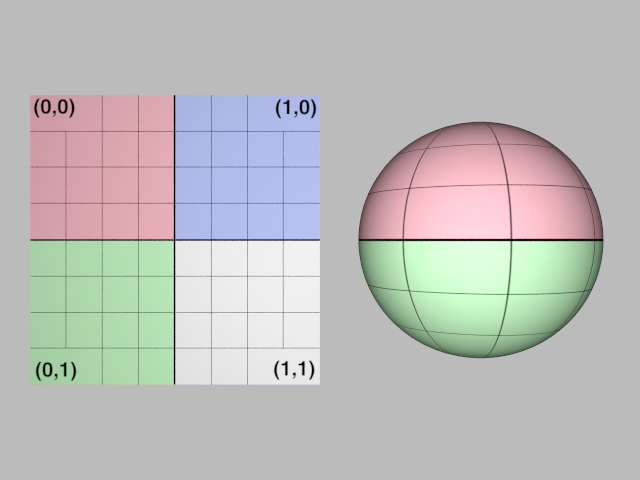
\includegraphics[width=0.19\linewidth]{imgs/hw_3_1a.png}
    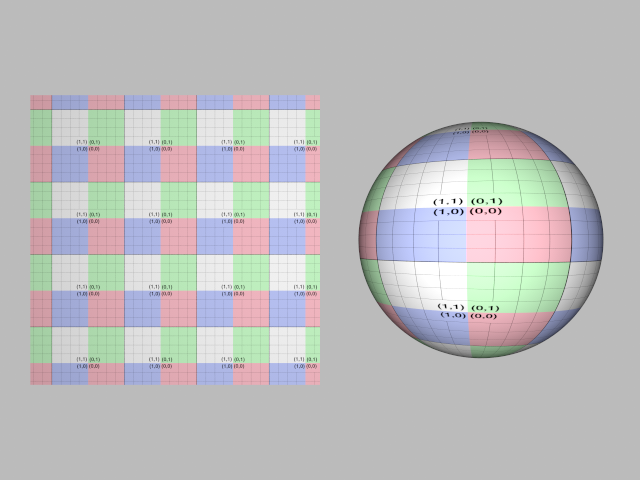
\includegraphics[width=0.19\linewidth]{imgs/hw_3_1b.png}
    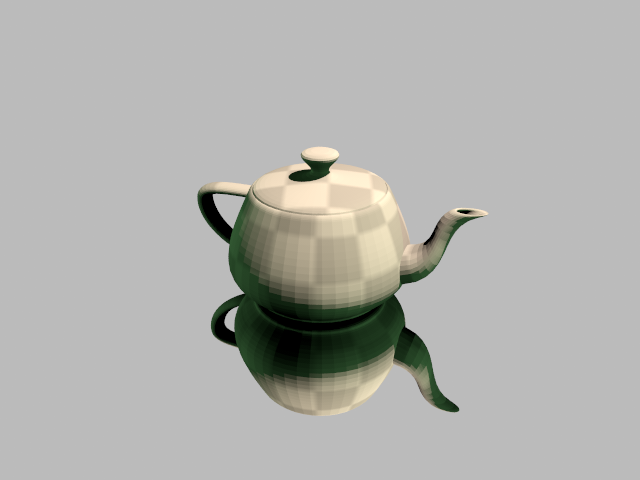
\includegraphics[width=0.19\linewidth]{imgs/hw_3_1c.png}
    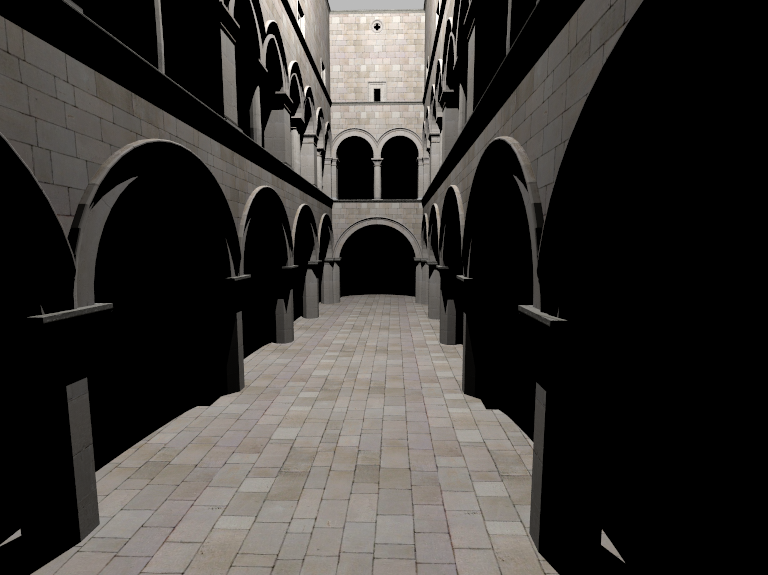
\includegraphics[width=0.19\linewidth]{imgs/hw_3_1d.png}
    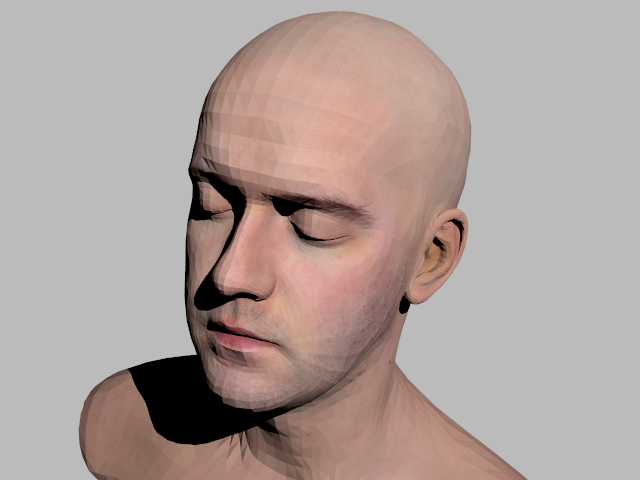
\includegraphics[width=0.19\linewidth]{imgs/hw_3_1e.png}
    \caption{Reference images for Homework 3.1.}
    \label{fig:hw_3_1}
\end{figure}

\section{Shading normals}
You have probably noticed that some of the 3D models we rendered look ``polygonal'', while we ideally want them to be smooth. One way to improve this is to increase the polygon count, but this approach seems expensive. \href{https://en.wikipedia.org/wiki/Phong_shading}{Phong} has come up with a genius way to make polygonal surfaces look smooth. The idea is to define a \emph{shading normal} per triangle vertex, and interpolate the normal within the triangle to have smooth normals. We will implement shading normals in this part.

Our \lstinline{ParsedTriangleMesh} can come with a field \lstinline{normals} which is its shading normals defined per-vertex (if \lstinline{ParsedTriangleMesh::normals.size() == 0}, then the mesh does not have shading normals). Once you hit a triangle, if it has a shading normal, interpolate the normals using the barycentric coordinates (just like how you interpolate the UV coordinates). Then, during shading, replace the normal you used with the interpolated shading normal.

%\bibliographystyle{plain}
%\bibliography{refs}

\end{document}
